% Image wrapper: PDF table structure was not recoverable automatically.
% Requires \usepackage{graphicx}. Replace the image with tabular cells when editable text is needed.
% Caption: Table XXXIV shows that increasing this coefficient raises computationaloverhead.Accuracyimproveswithincreasing factors, peaking at 0.6, but declines beyond this point; for exam- ple, a factor of 0.8 results in a performance drop. This degrada- tion is likely due to significant information loss introduced by the second linear layer. Therefore, maintaining a balanced channel reductionbetweenthetwolinearlayersismoreeffectivefor generating accurate attention weights. Three-scale or four-scale architecture? Following previous general and multi-task image restoration models [14], [15], [22], [25], [29], [62], [66], [104], [109], [141], we adopt a U-shaped architecturetoenableefficientmulti-scalelearning.Existing approachestypicallyemployeitherathree-scaleorfour-scale pipeline. The key difference between these two variants is that the additional deepest layer in the four-scale design introduces asubstantialnumberofparameters.Toinvestigatethisdesign choice, we conduct experiments using our small model and its four-scalecounterpart,withthenumberofblockssetto[3,3,
\begin{tabular}{c}
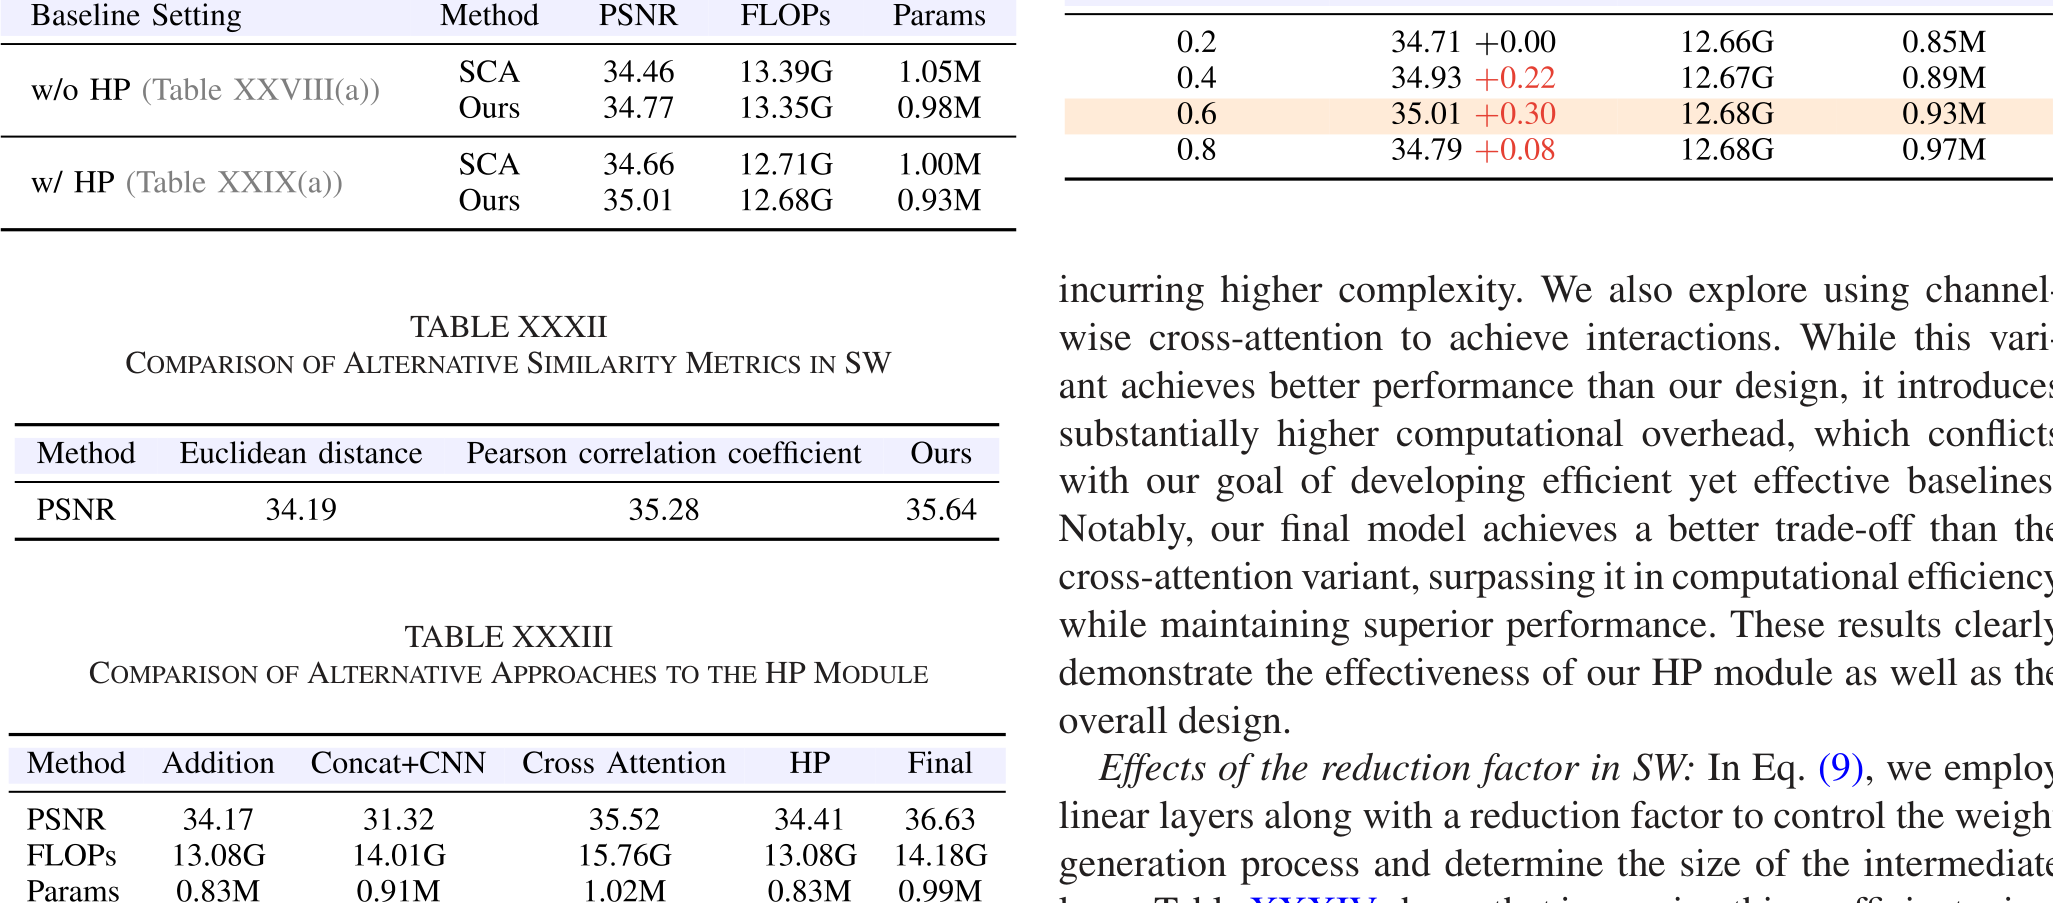
\includegraphics[width=\linewidth]{../original/Table34_p014.png}
\end{tabular}
